% Coarsest G2 Grassmannian cell 29: rays 13,14,17,18, orbit 30, with its rays clockwise from the top left corner; G2-trees with lettered inner vertices, generated by julia/to_tex/lettered_square_figure.jl
% Bounded edges of length 1.2677 in the cell and 1.3 in the rays, before scaling.
% Letters of the inner vertices of the rays, in the order of the rays:
%   A: the side {3,4,5,6,7} and {1,2,6,7} of its edges
%   B: the side {3,4,5} of its edges
%   C: the side {1,2} of its edges
%   D: the side {3,4,5,6,7} and {1,2,3,6,7} of its edges
%   E: the side {1,2} of its edges
%   F: the side {4,5} of its edges
%   G: the side {1,2,3,6,7} and {3,4,5,7} of its edges
%   H: the side {1,2,6} of its edges
%   I: the side {4,5} of its edges
%   J: the side {3,4,5,7} and {1,2,6,7} of its edges
%   K: the side {1,2,6} of its edges
%   L: the side {3,4,5} of its edges
\begingroup
\definecolor{g2RayLabel}{HTML}{000000}
\definecolor{g2CellLabel}{HTML}{000000}
\definecolor{g2TaxonBlue}{HTML}{1676A3}
\colorlet{g2SquareFill}{g2TaxonBlue!10}
\tikzset{
g2square side/.style={draw=g2RayLabel,line width=.8pt},
g2square circle/.style={draw=g2RayLabel,fill=white,line width=.8pt},
g2square cell/.style={fill=g2SquareFill},
g2square name/.style={text=g2RayLabel,inner sep=0pt,font=\boldmath},
g2square cell name/.style={g2square name,text=g2CellLabel},
  g2triangle letter/.style={text=g2RayLabel,inner sep=0pt,font={\sffamily\bfseries\fontsize{8}{8}\selectfont}},
}
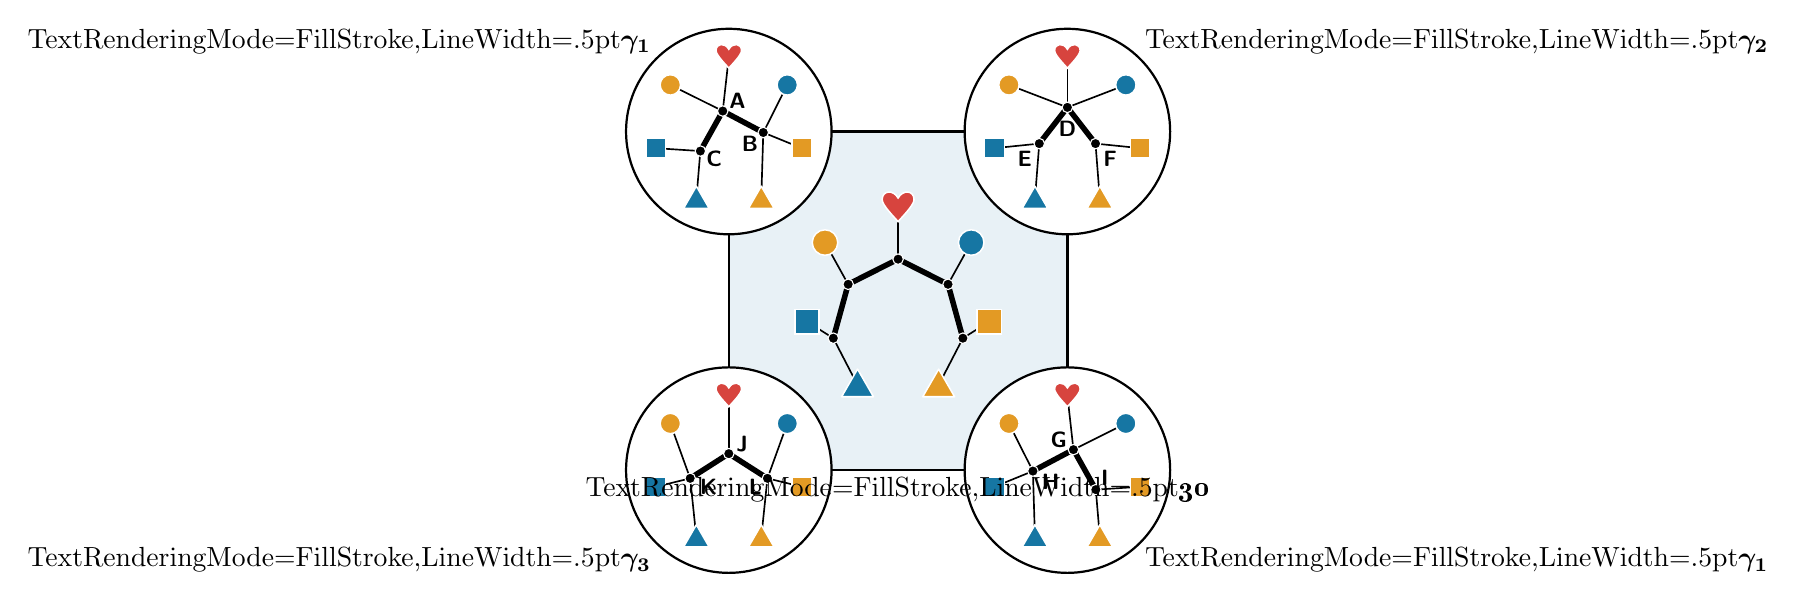
\begin{tikzpicture}[x=1cm,y=1cm,baseline=(current bounding box.center)]
\fill[g2square cell] (-2.15,2.15)--(2.15,2.15)--(2.15,-2.15)--(-2.15,-2.15)--cycle;
\draw[g2square side] (-2.15,2.15)--(2.15,2.15)--(2.15,-2.15)--(-2.15,-2.15)--cycle;
% Ray 13
\draw[g2square circle] (-2.15,2.15) circle[radius=1.305];
\node[g2square name,anchor=south east] at (-3.1293,3.1293) {\textpdfrender{TextRenderingMode=FillStroke,LineWidth=.5pt}{\bfseries\boldmath \(\gamma_1\)}};
\begin{scope}[shift={(-2.15,2.15)}]
\begingroup
\definecolor{g2TaxonBlue}{HTML}{1676A3}
\definecolor{g2TaxonYellow}{HTML}{E39A24}
\definecolor{g2HeartRed}{HTML}{D7443E}
\tikzset{
  g2tree pendant/.style={draw=black,line width=.6pt,line cap=round},
  g2tree internal/.style={draw=black,line width=2pt,line cap=round},
  g2tree vertex/.style={circle,fill=black,draw=white,line width=.4pt,inner sep=0pt,minimum size=3.8pt},
  g2tree dark/.style={fill=g2TaxonBlue,draw=white,line width=.55pt,text=white,inner sep=0pt},
  g2tree light/.style={fill=g2TaxonYellow,draw=white,line width=.55pt,text=white,inner sep=0pt},
  g2tree weight/.style={circle,fill=white,draw=none,text=black,inner sep=.15pt,minimum size=8.5pt},
  g2tree aligned pendant/.style={fill=white,text=black,inner sep=.7pt,sloped,above=1pt,font={\sffamily\fontsize{7.5}{8}\selectfont}},
  g2tree aligned internal/.style={fill=white,text=black,inner sep=1pt,sloped,above=1pt,font={\sffamily\fontsize{7.5}{8}\selectfont\bfseries}},
}
\coordinate (v1) at (-0.92595,-0.21134);
\coordinate (v2) at (-0.41209,-0.85570);
\coordinate (v3) at (0.74255,0.59217);
\coordinate (v4) at (0.92595,-0.21134);
\coordinate (v5) at (0.41209,-0.85570);
\coordinate (v6) at (-0.74255,0.59217);
\coordinate (v7) at (0.00000,0.94976);
\coordinate (v8) at (-0.36117,-0.24799);
\coordinate (v9) at (0.43794,-0.01225);
\coordinate (v10) at (-0.07677,0.26025);
\draw[g2tree internal] (v8)--(v10);
\draw[g2tree internal] (v9)--(v10);
\draw[g2tree pendant] (v1)--(v8);
\draw[g2tree pendant] (v2)--(v8);
\draw[g2tree pendant] (v3)--(v9);
\draw[g2tree pendant] (v4)--(v9);
\draw[g2tree pendant] (v5)--(v9);
\draw[g2tree pendant] (v6)--(v10);
\draw[g2tree pendant] (v7)--(v10);
\node[g2tree vertex] at (v8) {};
\node[g2tree vertex] at (v9) {};
\node[g2tree vertex] at (v10) {};
\node[g2tree dark,rectangle,minimum size=2.484mm,font={\sffamily\fontsize{4.8}{4.8}\selectfont\bfseries}] at (v1) {};
\begin{scope}[shift={(v2)},scale=0.54,transform shape]
\path[fill=g2TaxonBlue,draw=white,line width=.55pt,line join=round] (0mm,3.0mm)--(-3.0mm,-2.2mm)--(3.0mm,-2.2mm)--cycle;
\end{scope}
\node[g2tree dark,circle,minimum size=2.592mm,font={\sffamily\fontsize{4.8}{4.8}\selectfont\bfseries}] at (v3) {};
\node[g2tree light,rectangle,minimum size=2.484mm,font={\sffamily\fontsize{4.8}{4.8}\selectfont\bfseries}] at (v4) {};
\begin{scope}[shift={(v5)},scale=0.54,transform shape]
\path[fill=g2TaxonYellow,draw=white,line width=.55pt,line join=round] (0mm,3.0mm)--(-3.0mm,-2.2mm)--(3.0mm,-2.2mm)--cycle;
\end{scope}
\node[g2tree light,circle,minimum size=2.592mm,font={\sffamily\fontsize{4.8}{4.8}\selectfont\bfseries}] at (v6) {};
\begin{scope}[shift={(v7)},scale=0.54,transform shape]
\path[fill=g2HeartRed,draw=white,line width=.55pt]
  (0mm,-2.7mm)..controls(-.45mm,-2.1mm)and(-3.0mm,.35mm)..(-3.0mm,1.45mm)
  ..controls(-3.0mm,3.2mm)and(-.9mm,3.4mm)..(0mm,1.75mm)
  ..controls(.9mm,3.4mm)and(3.0mm,3.2mm)..(3.0mm,1.45mm)
  ..controls(3.0mm,.35mm)and(.45mm,-2.1mm)..(0mm,-2.7mm)--cycle;
\end{scope}
\node[g2triangle letter] at (-0.185,-0.35) {C};
\node[g2triangle letter] at (0.27,-0.15) {B};
\node[g2triangle letter] at (0.11,0.39) {A};
\endgroup
\end{scope}
% Ray 14
\draw[g2square circle] (2.15,2.15) circle[radius=1.305];
\node[g2square name,anchor=south west] at (3.1293,3.1293) {\textpdfrender{TextRenderingMode=FillStroke,LineWidth=.5pt}{\bfseries\boldmath \(\gamma_2\)}};
\begin{scope}[shift={(2.15,2.15)}]
\begingroup
\definecolor{g2TaxonBlue}{HTML}{1676A3}
\definecolor{g2TaxonYellow}{HTML}{E39A24}
\definecolor{g2HeartRed}{HTML}{D7443E}
\tikzset{
  g2tree pendant/.style={draw=black,line width=.6pt,line cap=round},
  g2tree internal/.style={draw=black,line width=2pt,line cap=round},
  g2tree vertex/.style={circle,fill=black,draw=white,line width=.4pt,inner sep=0pt,minimum size=3.8pt},
  g2tree dark/.style={fill=g2TaxonBlue,draw=white,line width=.55pt,text=white,inner sep=0pt},
  g2tree light/.style={fill=g2TaxonYellow,draw=white,line width=.55pt,text=white,inner sep=0pt},
  g2tree weight/.style={circle,fill=white,draw=none,text=black,inner sep=.15pt,minimum size=8.5pt},
  g2tree aligned pendant/.style={fill=white,text=black,inner sep=.7pt,sloped,above=1pt,font={\sffamily\fontsize{7.5}{8}\selectfont}},
  g2tree aligned internal/.style={fill=white,text=black,inner sep=1pt,sloped,above=1pt,font={\sffamily\fontsize{7.5}{8}\selectfont\bfseries}},
}
\coordinate (v1) at (-0.92595,-0.21134);
\coordinate (v2) at (-0.41209,-0.85570);
\coordinate (v3) at (0.74255,0.59217);
\coordinate (v4) at (0.92595,-0.21134);
\coordinate (v5) at (0.41209,-0.85570);
\coordinate (v6) at (-0.74255,0.59217);
\coordinate (v7) at (0.00000,0.94976);
\coordinate (v8) at (-0.35712,-0.15335);
\coordinate (v9) at (0.35712,-0.15335);
\coordinate (v10) at (0.00000,0.30670);
\draw[g2tree internal] (v8)--(v10);
\draw[g2tree internal] (v9)--(v10);
\draw[g2tree pendant] (v1)--(v8);
\draw[g2tree pendant] (v2)--(v8);
\draw[g2tree pendant] (v3)--(v10);
\draw[g2tree pendant] (v4)--(v9);
\draw[g2tree pendant] (v5)--(v9);
\draw[g2tree pendant] (v6)--(v10);
\draw[g2tree pendant] (v7)--(v10);
\node[g2tree vertex] at (v8) {};
\node[g2tree vertex] at (v9) {};
\node[g2tree vertex] at (v10) {};
\node[g2tree dark,rectangle,minimum size=2.484mm,font={\sffamily\fontsize{4.8}{4.8}\selectfont\bfseries}] at (v1) {};
\begin{scope}[shift={(v2)},scale=0.54,transform shape]
\path[fill=g2TaxonBlue,draw=white,line width=.55pt,line join=round] (0mm,3.0mm)--(-3.0mm,-2.2mm)--(3.0mm,-2.2mm)--cycle;
\end{scope}
\node[g2tree dark,circle,minimum size=2.592mm,font={\sffamily\fontsize{4.8}{4.8}\selectfont\bfseries}] at (v3) {};
\node[g2tree light,rectangle,minimum size=2.484mm,font={\sffamily\fontsize{4.8}{4.8}\selectfont\bfseries}] at (v4) {};
\begin{scope}[shift={(v5)},scale=0.54,transform shape]
\path[fill=g2TaxonYellow,draw=white,line width=.55pt,line join=round] (0mm,3.0mm)--(-3.0mm,-2.2mm)--(3.0mm,-2.2mm)--cycle;
\end{scope}
\node[g2tree light,circle,minimum size=2.592mm,font={\sffamily\fontsize{4.8}{4.8}\selectfont\bfseries}] at (v6) {};
\begin{scope}[shift={(v7)},scale=0.54,transform shape]
\path[fill=g2HeartRed,draw=white,line width=.55pt]
  (0mm,-2.7mm)..controls(-.45mm,-2.1mm)and(-3.0mm,.35mm)..(-3.0mm,1.45mm)
  ..controls(-3.0mm,3.2mm)and(-.9mm,3.4mm)..(0mm,1.75mm)
  ..controls(.9mm,3.4mm)and(3.0mm,3.2mm)..(3.0mm,1.45mm)
  ..controls(3.0mm,.35mm)and(.45mm,-2.1mm)..(0mm,-2.7mm)--cycle;
\end{scope}
\node[g2triangle letter] at (-0.5421,-0.3427) {E};
\node[g2triangle letter] at (0.5421,-0.3427) {F};
\node[g2triangle letter] at (0.0,0.0301) {D};
\endgroup
\end{scope}
% Ray 17
\draw[g2square circle] (2.15,-2.15) circle[radius=1.305];
\node[g2square name,anchor=north west] at (3.1293,-3.1293) {\textpdfrender{TextRenderingMode=FillStroke,LineWidth=.5pt}{\bfseries\boldmath \(\gamma_1\)}};
\begin{scope}[shift={(2.15,-2.15)}]
\begingroup
\definecolor{g2TaxonBlue}{HTML}{1676A3}
\definecolor{g2TaxonYellow}{HTML}{E39A24}
\definecolor{g2HeartRed}{HTML}{D7443E}
\tikzset{
  g2tree pendant/.style={draw=black,line width=.6pt,line cap=round},
  g2tree internal/.style={draw=black,line width=2pt,line cap=round},
  g2tree vertex/.style={circle,fill=black,draw=white,line width=.4pt,inner sep=0pt,minimum size=3.8pt},
  g2tree dark/.style={fill=g2TaxonBlue,draw=white,line width=.55pt,text=white,inner sep=0pt},
  g2tree light/.style={fill=g2TaxonYellow,draw=white,line width=.55pt,text=white,inner sep=0pt},
  g2tree weight/.style={circle,fill=white,draw=none,text=black,inner sep=.15pt,minimum size=8.5pt},
  g2tree aligned pendant/.style={fill=white,text=black,inner sep=.7pt,sloped,above=1pt,font={\sffamily\fontsize{7.5}{8}\selectfont}},
  g2tree aligned internal/.style={fill=white,text=black,inner sep=1pt,sloped,above=1pt,font={\sffamily\fontsize{7.5}{8}\selectfont\bfseries}},
}
\coordinate (v1) at (-0.92595,-0.21134);
\coordinate (v2) at (-0.41209,-0.85570);
\coordinate (v3) at (0.74255,0.59217);
\coordinate (v4) at (0.92595,-0.21134);
\coordinate (v5) at (0.41209,-0.85570);
\coordinate (v6) at (-0.74255,0.59217);
\coordinate (v7) at (0.00000,0.94976);
\coordinate (v8) at (0.36117,-0.24799);
\coordinate (v9) at (-0.43794,-0.01225);
\coordinate (v10) at (0.07677,0.26025);
\draw[g2tree internal] (v8)--(v10);
\draw[g2tree internal] (v9)--(v10);
\draw[g2tree pendant] (v1)--(v9);
\draw[g2tree pendant] (v2)--(v9);
\draw[g2tree pendant] (v3)--(v10);
\draw[g2tree pendant] (v4)--(v8);
\draw[g2tree pendant] (v5)--(v8);
\draw[g2tree pendant] (v6)--(v9);
\draw[g2tree pendant] (v7)--(v10);
\node[g2tree vertex] at (v8) {};
\node[g2tree vertex] at (v9) {};
\node[g2tree vertex] at (v10) {};
\node[g2tree dark,rectangle,minimum size=2.484mm,font={\sffamily\fontsize{4.8}{4.8}\selectfont\bfseries}] at (v1) {};
\begin{scope}[shift={(v2)},scale=0.54,transform shape]
\path[fill=g2TaxonBlue,draw=white,line width=.55pt,line join=round] (0mm,3.0mm)--(-3.0mm,-2.2mm)--(3.0mm,-2.2mm)--cycle;
\end{scope}
\node[g2tree dark,circle,minimum size=2.592mm,font={\sffamily\fontsize{4.8}{4.8}\selectfont\bfseries}] at (v3) {};
\node[g2tree light,rectangle,minimum size=2.484mm,font={\sffamily\fontsize{4.8}{4.8}\selectfont\bfseries}] at (v4) {};
\begin{scope}[shift={(v5)},scale=0.54,transform shape]
\path[fill=g2TaxonYellow,draw=white,line width=.55pt,line join=round] (0mm,3.0mm)--(-3.0mm,-2.2mm)--(3.0mm,-2.2mm)--cycle;
\end{scope}
\node[g2tree light,circle,minimum size=2.592mm,font={\sffamily\fontsize{4.8}{4.8}\selectfont\bfseries}] at (v6) {};
\begin{scope}[shift={(v7)},scale=0.54,transform shape]
\path[fill=g2HeartRed,draw=white,line width=.55pt]
  (0mm,-2.7mm)..controls(-.45mm,-2.1mm)and(-3.0mm,.35mm)..(-3.0mm,1.45mm)
  ..controls(-3.0mm,3.2mm)and(-.9mm,3.4mm)..(0mm,1.75mm)
  ..controls(.9mm,3.4mm)and(3.0mm,3.2mm)..(3.0mm,1.45mm)
  ..controls(3.0mm,.35mm)and(.45mm,-2.1mm)..(0mm,-2.7mm)--cycle;
\end{scope}
\node[g2triangle letter] at (0.475,-0.095) {I};
\node[g2triangle letter] at (-0.2123,-0.1434) {H};
\node[g2triangle letter] at (-0.11,0.39) {G};
\endgroup
\end{scope}
% Ray 18
\draw[g2square circle] (-2.15,-2.15) circle[radius=1.305];
\node[g2square name,anchor=north east] at (-3.1293,-3.1293) {\textpdfrender{TextRenderingMode=FillStroke,LineWidth=.5pt}{\bfseries\boldmath \(\gamma_3\)}};
\begin{scope}[shift={(-2.15,-2.15)}]
\begingroup
\definecolor{g2TaxonBlue}{HTML}{1676A3}
\definecolor{g2TaxonYellow}{HTML}{E39A24}
\definecolor{g2HeartRed}{HTML}{D7443E}
\tikzset{
  g2tree pendant/.style={draw=black,line width=.6pt,line cap=round},
  g2tree internal/.style={draw=black,line width=2pt,line cap=round},
  g2tree vertex/.style={circle,fill=black,draw=white,line width=.4pt,inner sep=0pt,minimum size=3.8pt},
  g2tree dark/.style={fill=g2TaxonBlue,draw=white,line width=.55pt,text=white,inner sep=0pt},
  g2tree light/.style={fill=g2TaxonYellow,draw=white,line width=.55pt,text=white,inner sep=0pt},
  g2tree weight/.style={circle,fill=white,draw=none,text=black,inner sep=.15pt,minimum size=8.5pt},
  g2tree aligned pendant/.style={fill=white,text=black,inner sep=.7pt,sloped,above=1pt,font={\sffamily\fontsize{7.5}{8}\selectfont}},
  g2tree aligned internal/.style={fill=white,text=black,inner sep=1pt,sloped,above=1pt,font={\sffamily\fontsize{7.5}{8}\selectfont\bfseries}},
}
\coordinate (v1) at (-0.92595,-0.21134);
\coordinate (v2) at (-0.41209,-0.85570);
\coordinate (v3) at (0.74255,0.59217);
\coordinate (v4) at (0.92595,-0.21134);
\coordinate (v5) at (0.41209,-0.85570);
\coordinate (v6) at (-0.74255,0.59217);
\coordinate (v7) at (0.00000,0.94976);
\coordinate (v8) at (-0.49074,-0.10454);
\coordinate (v9) at (0.00000,0.20908);
\coordinate (v10) at (0.49074,-0.10454);
\draw[g2tree internal] (v8)--(v9);
\draw[g2tree internal] (v9)--(v10);
\draw[g2tree pendant] (v1)--(v8);
\draw[g2tree pendant] (v2)--(v8);
\draw[g2tree pendant] (v3)--(v10);
\draw[g2tree pendant] (v4)--(v10);
\draw[g2tree pendant] (v5)--(v10);
\draw[g2tree pendant] (v6)--(v8);
\draw[g2tree pendant] (v7)--(v9);
\node[g2tree vertex] at (v8) {};
\node[g2tree vertex] at (v9) {};
\node[g2tree vertex] at (v10) {};
\node[g2tree dark,rectangle,minimum size=2.484mm,font={\sffamily\fontsize{4.8}{4.8}\selectfont\bfseries}] at (v1) {};
\begin{scope}[shift={(v2)},scale=0.54,transform shape]
\path[fill=g2TaxonBlue,draw=white,line width=.55pt,line join=round] (0mm,3.0mm)--(-3.0mm,-2.2mm)--(3.0mm,-2.2mm)--cycle;
\end{scope}
\node[g2tree dark,circle,minimum size=2.592mm,font={\sffamily\fontsize{4.8}{4.8}\selectfont\bfseries}] at (v3) {};
\node[g2tree light,rectangle,minimum size=2.484mm,font={\sffamily\fontsize{4.8}{4.8}\selectfont\bfseries}] at (v4) {};
\begin{scope}[shift={(v5)},scale=0.54,transform shape]
\path[fill=g2TaxonYellow,draw=white,line width=.55pt,line join=round] (0mm,3.0mm)--(-3.0mm,-2.2mm)--(3.0mm,-2.2mm)--cycle;
\end{scope}
\node[g2tree light,circle,minimum size=2.592mm,font={\sffamily\fontsize{4.8}{4.8}\selectfont\bfseries}] at (v6) {};
\begin{scope}[shift={(v7)},scale=0.54,transform shape]
\path[fill=g2HeartRed,draw=white,line width=.55pt]
  (0mm,-2.7mm)..controls(-.45mm,-2.1mm)and(-3.0mm,.35mm)..(-3.0mm,1.45mm)
  ..controls(-3.0mm,3.2mm)and(-.9mm,3.4mm)..(0mm,1.75mm)
  ..controls(.9mm,3.4mm)and(3.0mm,3.2mm)..(3.0mm,1.45mm)
  ..controls(3.0mm,.35mm)and(.45mm,-2.1mm)..(0mm,-2.7mm)--cycle;
\end{scope}
\node[g2triangle letter] at (-0.2556,-0.2178) {K};
\node[g2triangle letter] at (0.17,0.33) {J};
\node[g2triangle letter] at (0.335,-0.215) {L};
\endgroup
\end{scope}
% The cell
\node[g2square cell name,anchor=north] at (0.0,-2.23) {\textpdfrender{TextRenderingMode=FillStroke,LineWidth=.5pt}{\bfseries\boldmath \oldstylenums{30}}};
\begingroup
\definecolor{g2TaxonBlue}{HTML}{1676A3}
\definecolor{g2TaxonYellow}{HTML}{E39A24}
\definecolor{g2HeartRed}{HTML}{D7443E}
\tikzset{
  g2tree pendant/.style={draw=black,line width=.6pt,line cap=round},
  g2tree internal/.style={draw=black,line width=2pt,line cap=round},
  g2tree vertex/.style={circle,fill=black,draw=white,line width=.4pt,inner sep=0pt,minimum size=3.8pt},
  g2tree dark/.style={fill=g2TaxonBlue,draw=white,line width=.55pt,text=white,inner sep=0pt},
  g2tree light/.style={fill=g2TaxonYellow,draw=white,line width=.55pt,text=white,inner sep=0pt},
  g2tree weight/.style={circle,fill=white,draw=none,text=black,inner sep=.15pt,minimum size=8.5pt},
  g2tree aligned pendant/.style={fill=white,text=black,inner sep=.7pt,sloped,above=1pt,font={\sffamily\fontsize{7.5}{8}\selectfont}},
  g2tree aligned internal/.style={fill=white,text=black,inner sep=1pt,sloped,above=1pt,font={\sffamily\fontsize{7.5}{8}\selectfont\bfseries}},
}
\coordinate (v1) at (-1.15743,-0.26418);
\coordinate (v2) at (-0.51511,-1.06963);
\coordinate (v3) at (0.92819,0.74021);
\coordinate (v4) at (1.15743,-0.26418);
\coordinate (v5) at (0.51511,-1.06963);
\coordinate (v6) at (-0.92819,0.74021);
\coordinate (v7) at (0.00000,1.18720);
\coordinate (v8) at (-0.82275,-0.47448);
\coordinate (v9) at (0.82275,-0.47448);
\coordinate (v10) at (0.63408,0.20991);
\coordinate (v11) at (-0.63408,0.20991);
\coordinate (v12) at (0.00000,0.52916);
\draw[g2tree internal] (v8)--(v11);
\draw[g2tree internal] (v9)--(v10);
\draw[g2tree internal] (v10)--(v12);
\draw[g2tree internal] (v11)--(v12);
\draw[g2tree pendant] (v1)--(v8);
\draw[g2tree pendant] (v2)--(v8);
\draw[g2tree pendant] (v3)--(v10);
\draw[g2tree pendant] (v4)--(v9);
\draw[g2tree pendant] (v5)--(v9);
\draw[g2tree pendant] (v6)--(v11);
\draw[g2tree pendant] (v7)--(v12);
\node[g2tree vertex] at (v8) {};
\node[g2tree vertex] at (v9) {};
\node[g2tree vertex] at (v10) {};
\node[g2tree vertex] at (v11) {};
\node[g2tree vertex] at (v12) {};
\node[g2tree dark,rectangle,minimum size=3.105mm,font={\sffamily\fontsize{6}{6}\selectfont\bfseries}] at (v1) {};
\begin{scope}[shift={(v2)},scale=0.675,transform shape]
\path[fill=g2TaxonBlue,draw=white,line width=.55pt,line join=round] (0mm,3.0mm)--(-3.0mm,-2.2mm)--(3.0mm,-2.2mm)--cycle;
\end{scope}
\node[g2tree dark,circle,minimum size=3.24mm,font={\sffamily\fontsize{6}{6}\selectfont\bfseries}] at (v3) {};
\node[g2tree light,rectangle,minimum size=3.105mm,font={\sffamily\fontsize{6}{6}\selectfont\bfseries}] at (v4) {};
\begin{scope}[shift={(v5)},scale=0.675,transform shape]
\path[fill=g2TaxonYellow,draw=white,line width=.55pt,line join=round] (0mm,3.0mm)--(-3.0mm,-2.2mm)--(3.0mm,-2.2mm)--cycle;
\end{scope}
\node[g2tree light,circle,minimum size=3.24mm,font={\sffamily\fontsize{6}{6}\selectfont\bfseries}] at (v6) {};
\begin{scope}[shift={(v7)},scale=0.675,transform shape]
\path[fill=g2HeartRed,draw=white,line width=.55pt]
  (0mm,-2.7mm)..controls(-.45mm,-2.1mm)and(-3.0mm,.35mm)..(-3.0mm,1.45mm)
  ..controls(-3.0mm,3.2mm)and(-.9mm,3.4mm)..(0mm,1.75mm)
  ..controls(.9mm,3.4mm)and(3.0mm,3.2mm)..(3.0mm,1.45mm)
  ..controls(3.0mm,.35mm)and(.45mm,-2.1mm)..(0mm,-2.7mm)--cycle;
\end{scope}
\endgroup
\ifdefined\gtwocelloverlay\gtwocelloverlay\fi
\end{tikzpicture}
\endgroup
